% This is samplepaper.tex, a sample chapter demonstrating the
% LLNCS macro package for Springer Computer Science proceedings;
% Version 2.20 of 2017/10/04
%
\documentclass[runningheads]{llncs}
%
\usepackage{graphicx}
\usepackage{tikz,pgfplots}
\usepackage{pgf-pie}  
\usepackage{subcaption}
\usepackage{hyperref}
\usepackage[autostyle]{csquotes}
\usepackage[%
  backend=biber,
  url=true,
  style=numeric, % alphabetic, numeric
  sorting=none, % default == nty, https://tex.stackexchange.com/questions/51434/biblatex-citation-order
  maxnames=1,
  minnames=1,
  maxbibnames=99,
  giveninits,
  uniquename=init]{biblatex}
% Used for displaying a sample figure. If possible, figure files should
% be included in EPS format.
%
% If you use the hyperref package, please uncomment the following line
% to display URLs in blue roman font according to Springer's eBook style:
% \renewcommand\UrlFont{\color{blue}\rmfamily}

\bibliography{zotero2}
\begin{document}
%
\title{Process and Blockchain \protect\\
  A Systematic Review}
%\thanks{Supported by organization x.}
%\titlerunning{Abbreviated paper title}
% If the paper title is too long for the running head, you can set
% an abbreviated paper title here
%
\author{Denis Paluca}
%
%\authorrunning{F. Author et al.}
% First names are abbreviated in the running head.
% If there are more than two authors, 'et al.' is used.
%
\institute{Technical University of Munich, Arcisstraße 21, 80333 Munich, Germany \email{denis.paluca@tum.de}}
%
\maketitle              % typeset the header of the contribution
%
\begin{abstract}
  Blockchain technology has been proposed as a solution for business process management (BPM). In this context, the capabilities of blockchain can facilitate cross-organizational collaborative business processes. Despite the potential benefits, there are numerous challenges associated with the implementation of collaborative processes using blockchain. But, the potential of this technology has led many studies to be conducted in this topic. In this work, we review the current literature to understand the solutions offered by the research field to address these challenges. For this systematic literature review (SLR), 13 papers were selected from more than 1600 identified studies. The review focuses on recent improvements in four key areas: trust awareness, flexibility, temporal constraints, and process design. Overall, the findings of this review highlight the benefits of integrating blockchain into BPM, new challenges and the need for further research in this area.

  \keywords{Blockchain  \and Business Process Management \and Literature Review}
\end{abstract}
%
%
%


\section{Introduction}
In recent years inter-organizational collaboration has become more and more common, with BPM having to undergo significant development according to technological advances \cite{ARIOUAT2017703}. This has put pressure on enterprises to improve their business processes by enabling dynamic collaborations among business partners. But, without central control these changes have proven too difficult to implement. When multiple parties are involved a trust mechanism is required in order to discourage malicious actors. In this context, blockchain has been suggested as a solution \cite{garcia-garcia_using_2020}.

Blockchain technology enables the automation of business processes and inter-organizational collaboration without the need for intermediaries. Traditionally, third parties act as intermediaries in business collaborations, but with blockchain, the immutability and transparency of the system allow for real-time auditing of process steps by business partners or regulatory authorities \cite{garcia-garcia_using_2020}. The data recorded through these business processes is permanent and unalterable, providing a trustworthy solution for companies engaging in collaboration. The tamper-proof nature of blockchain records further tackles the trust issue that companies may face in these situations.

This SLR aims to explore the relationship between blockchain, BPM, and collaborative processes. Here, we consider the most recent advancements made to the field by reviewing publications until November 2022. We selected 13 papers and showed how the proposed approaches handle challenges with BPM in a collaborative setting. We classify the papers on four key areas: trust awareness, flexibility, temporal constraints, and process design. By investigating the impact of blockchain on these areas, this review seeks to provide a comprehensive understanding of how blockchain can enhance BPM and inter-organizational collaborative processes. Additionally, the review will also provide insights into new challenges and future research directions.

% The results of this review have important implications for organizations, researchers, and policymakers. Organizations can use the findings of this review to make informed decisions on the adoption and implementation of blockchain technology in their BPM and inter-organizational collaborative processes. Researchers can use the review to identify the research gaps and opportunities in this area. Policymakers can use the review to understand the potential impact of blockchain on BPM and inter-organizational collaborative processes and formulate relevant policies to facilitate the adoption of blockchain.

% Overall, the purpose of this systematic literature review is to provide a comprehensive understanding of the relationship between blockchain, BPM, and inter-organizational collaborative processes and its impact on trust awareness, flexibility, temporal constraints, and process design.
 

% In open environments, sensitive data flows across distributed stakeholders, which raises concerns about security and privacy. Conventional BPM tools centralize controls of data flows and executions of BPs to ensure overall security and privacy. However, centralized control can be vulnerable to single points of failure and can be compromised if the executer of a BP becomes malicious. This lack of trust creates hesitation in BP participation and subsequently hinders the wide use of services. Furthermore, centralized BPM has some unsatisfactory performance such as latency and messaging delay.

% On the other hand, when BPs are distributed and decentralized, an adopted BPM tool must be flexible to deal with changes, dynamics, and uncertainties of business processes and stakeholders, and scalable to manage and execute BPs successfully when the number of available online services is changing dynamically. The challenges to BPM were briefed below with a comprehensive elaboration in section III and IV.

% \begin{enumerate}
%     \item In centralized BPM, a sole entity has full control of BP executions; business partners are obligated to trust this entity for task executions and data protection.
%     \item In decentralized BPM, the ownership of a BP is shared. No entity acquires full authority of entire BP executions. Each partner is allowed to access and process information under assigned responsibilities. Thus, it is necessary for BPM to monitor and validate executions during runtime.
%     \item With a rapid growth of IoT, many researchers argue that BC would be widely adopted to manage IoT-enabled business processes cost-effectively. Therefore, BPs will involve greater BC-based services. Mechanisms to assure trust of such services among disparate partners become an essential element of modern BPM.
%     \item Proprietary and heterogeneity of services are the main causes of inconsistency and incompatibility, hindering interoperations in a large scale.
%     \item The implementations of BC-based services are heterogeneous, implying different costs, performances, and delays to process and confirm BC transactions. Utilizing the services needs to be well justified to address these variants as well as uncertainties. For example, undesired consequences of time delays in a time-sensitive BP should be seriously addressed.
% \end{enumerate}

% Assuring trust of information inside BP interoperations is one of the critical requirements in modern BPM, and trust assurances are also required in the execution of tasks. Since BPM tends to be decentralized, BC is naturally considered as the appropriate mechanism to establish a trust repository among partners. Additionally, BC-based applications can offer auxiliary functions to assist BPM. BC technology has brought numerous opportunities to advance BPMs. It was originated as a technology underlying cryptocurrencies but its application has been extended to various domains such as supply chain management, healthcare, and finance.

% This SLR aims to provide a comprehensive understanding of the current state of research on this topic, and to identify areas for future research.

\subsection{Related work and Previous SLRs}
This work is based on the work of previous SLRs. Therefore, we intend to use these SLRs as a starting point and only focus in the most recent work. \citeauthor{frizzo-barker_blockchain_2020} \cite{frizzo-barker_blockchain_2020} investigated all studies connecting business scholarship to blockchain until the end of 2018. During the same time period, \citeauthor{mendling_blockchains_2018} \cite{mendling_blockchains_2018} published one of the most cited works which studies the challenges of blockchain in BPM. The SLR presented by \citeauthor{garcia-garcia_using_2020} \cite{garcia-garcia_using_2020} explores the application of blockchain in collaborative business processes. Another review by \citeauthor{lauster} \cite{lauster} groups studies relevant to blockchain and BPM into three topic clusters, namely application areas and challenges, process architecture and design, and execution related publications. In contrast to these works, we present areas where the capabilities of blockchain solutions have either been effectively utilized or enhanced to meet different demands of BPM.
\section{Methodology}
For our research we adopted the SLR method, so that we can analyze the relevant literature. SLRs are designed to provide an overview of the existing literature on a specific topic area ~\cite{frizzo-barker_blockchain_2020}. They are commonly used in the medical field and have been increasingly adopted by scientists as a tool in emerging fields.

\subsection{Research Questions}
Firstly, we define a set of research questions which help to narrow the wide topic of "Process and Blockchain". The following research questions were used as a guide to further examine the role blockchain can play in BPM.
\begin{enumerate}
    \item \textbf{How can BPM take advantage of blockchain technologies?} 
    
    %This question was laid out to identify the potential benefits and opportunities that blockchain technologies can bring to the field of business process management. By investigating the ways in which blockchain can optimize and streamline processes, this question can provide valuable insights into how companies can improve their operations and gain a competitive advantage.
    
    \item \textbf{What are the top challenges and risks associated with integrating blockchain in BPM?}
    
    %With this question we highlight the potential drawbacks and obstacles that companies may encounter when incorporating blockchain technologies into their operations. By identifying these challenges and risks, this question can provide guidance on how to mitigate them and ensure the successful implementation of blockchain in business process management.
    
    \item \textbf{Which applications of blockchain in BPM have been proposed and how are they evaluated?}

    %Providing an overview of the different ways in which blockchain technologies have been applied in the field of business process management is beneficial in deciding where future research and development efforts should be directed. By identifying the various proposals for blockchain-based solutions and evaluating their effectiveness, this question can give an insight into the state of the art of blockchain in BPM and provide a basis for future research.
\end{enumerate}

\subsection{Search Strategy}
Next, it is important to use a comprehensive search strategy in order to identify relevant studies. In this case, the databases chosen are IEEExplore, ScienceDirect, Springer Link and ACM Digital Library. These databases are widely used in academic research and are likely to contain relevant and high quality studies on the topic of blockchain in BPM. 
\setlength{\tabcolsep}{3em}
\begin{table}[]
    \centering
    \caption{Search keywords}
    \begin{tabular}{l r}
        \hline
        A & B \\
        \hline\hline
        Blockchain & Business Process\\
        Distributed Ledger &  Business Process Management\\
        DLT & BPM \\
        Smart contract &  \\
        Ethereum & \\
        \hline
    \end{tabular}
    \label{tab:keywords}
\end{table}

A combination of the search terms seen in Table \ref{tab:keywords} above were used to create the search string. Most databases we searched allowed using the logical operators (such as AND, OR, NOT) to combine all the terms in one search string and therefore avoid duplications.  The final search string was "(blockchain OR distributed ledger OR DLT OR smart contract OR ethereum) AND (business process OR business process management OR BPM)". Using the search string, we conducted a search in each of the selected databases. The search was conducted on November 2022 by using the following fields: title, abstract, and keywords. We already limited our search to English studies published between 2020 and 2022, according to our study selection criteria further explained in \ref{ssec:study-selection}. At this stage, the search resulted in 1659 documents being identified.

\subsection{Study Selection} \label{ssec:study-selection}
In the third phase, we use different selection criteria to define the parameters of the studies that will be included in the SLR. Applying these criteria makes sure that we identified studies with high relevance and quality. Studies were included if they fulfilled at least one of the following inclusion criteria:
\begin{enumerate}
    \item Studies that examine the use of blockchain in the BPM lifecycle.
    \item Studies that present a new solution to integrating blockchain in BPM.
    \item Studies that extends a blockchain-based solution for BPM.
\end{enumerate}

%To ensure a focus on high-quality work, some articles that were deemed irrelevant, low-quality, or of low importance were removed. 
\noindent The following were the exclusion criteria used to discard irrelevant studies.
\begin{enumerate}
    \item Studies not written in English.
    \item Studies not published between 2020 and 2022.
    \item Studies with no reviewers.
    \item Non primary studies.
    \item Studies which handle a specific application area (such as supply chain management) and are not intended for BPs and BPM in general.
\end{enumerate}
To implement the criteria, we first filtered the results by reading the title which reduced the documents from 1659 to 71 potential papers. Then, by reading the abstract and skimming through the key contents of the papers we reduced this number further down to 11. Searching the citations yielded two different papers bringing the total of selected studies to 13.

\begin{figure}
    \centering
    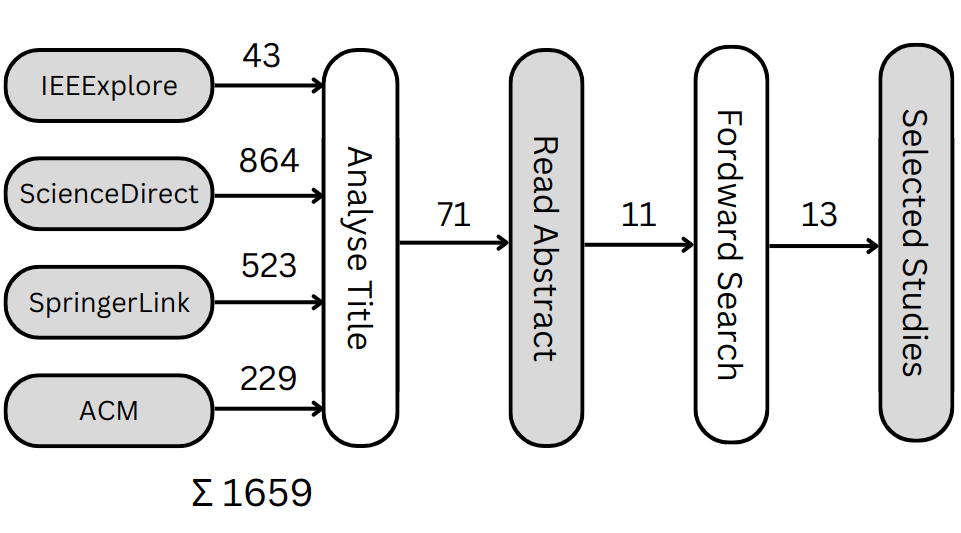
\includegraphics[width=\textwidth]{search-final.png}
    \caption{Search timeline}
    \label{fig:search}
\end{figure}
\section{Results}
\subsection{Quantitative analysis}
In this section, we present a quantitative analysis of the results from the studies that were included in the review. The objective of this analysis is to provide an overview of the distribution of authors across different countries and continents (Fig. \ref{fig:geo}), the type of research conducted (Fig. \ref{fig:concept}), and the blockchain technologies employed for each study (Fig. \ref{fig:blockchain}).

\begin{figure}
\centering
\begin{subfigure}{.5\textwidth}
    \centering
    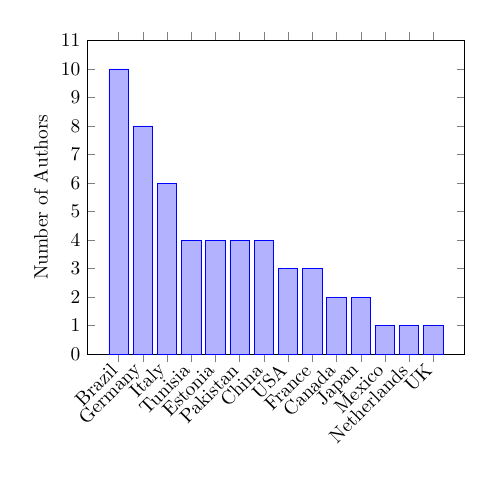
\begin{tikzpicture}[scale=0.7, transform shape]
    \begin{axis}[
        ybar, % create a bar chart
        ylabel={Number of Authors}, % label for the y-axis
        xtick=data, % display tick marks for each data point
        xticklabels={Brazil,Germany,Italy,Tunisia,Estonia,Pakistan,China,USA,France,Canada,Japan,Mexico,Netherlands,UK}, % display the country names for each tick mark
        ymin=0, % set the minimum value for the y-axis to 0
        ymax=11, % set the maximum value for the y-axis to 4
        ytick={0,1,2,3,4,5,6,7,8,9,10,11}, % display tick marks for each integer value on the y-axis
        xticklabel style={rotate=45, anchor=east}, % rotate x-tick labels by 45 degrees and align them to the east
    ]
    \addplot coordinates {(1,10) (2,8) (3,6) (4,4) (5,4) (6,4) (7,4) (8,3) (9,3) (10,2) (11,2) (12,1) (13,1) (14,1)}; % plot the data
    \end{axis}
    \end{tikzpicture}
    \caption{By country}
    \label{fig:geo-country}
\end{subfigure}%
\begin{subfigure}{.5\textwidth}
    \centering
    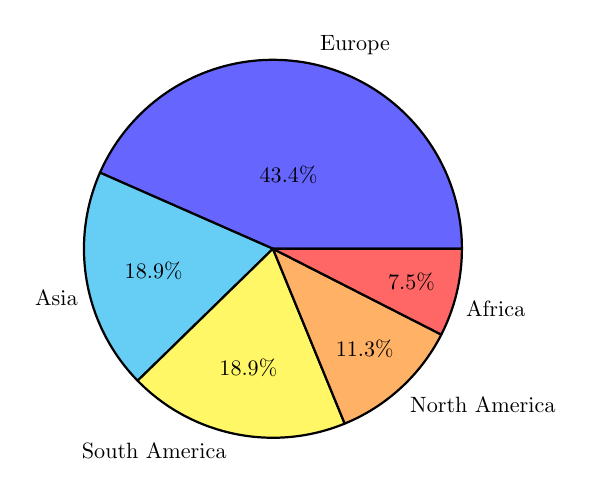
\begin{tikzpicture}[scale=0.8, transform shape]
    \pie{43.4/Europe,
        18.9/Asia,
        18.9/South America,
        11.3/North America,
        7.5/Africa}
    \end{tikzpicture}
    \caption{By continent}
    \label{fig:geo-continent}
\end{subfigure}%
\caption{Geographic distribution of authors}
\label{fig:geo}
\end{figure}

The intersection between blockchain and BPM has gained interest from multiple nations, with authors based in 14 countries contributing to its research. As can be seen in Fig. \ref{fig:geo-country}, the majority authors were based in the Brazil (10, 18.9\%) followed by the Germany (8, 15.1\%) and Italy (6, 11.3\%), then Tunisia, Estonia, Pakistan, and China (11 each, 7\%). The remaining countries had 3 or less authors who contributed to the selected studies. Brazil in this case is an outlier with 10 authors only working on \citeauthor{alves_exploring_2022} \cite{alves_exploring_2022}. In contrast to the 6 authors from Italy who contributed to both \citeauthor{corradini_engineering_2022} \cite{corradini_engineering_2022} and \citeauthor{corradini_flexible_2022} \cite{corradini_flexible_2022}. The research is mostly concentrated in Europe (43.4\%), Asia and South America (18.9\% each) while North America has 11.3\% as seen in Fig. \ref{fig:geo-continent}. The regions with the least representation are Africa (7.5\%) and Australia with no authors.
\begin{figure}[!h]
    \centering
    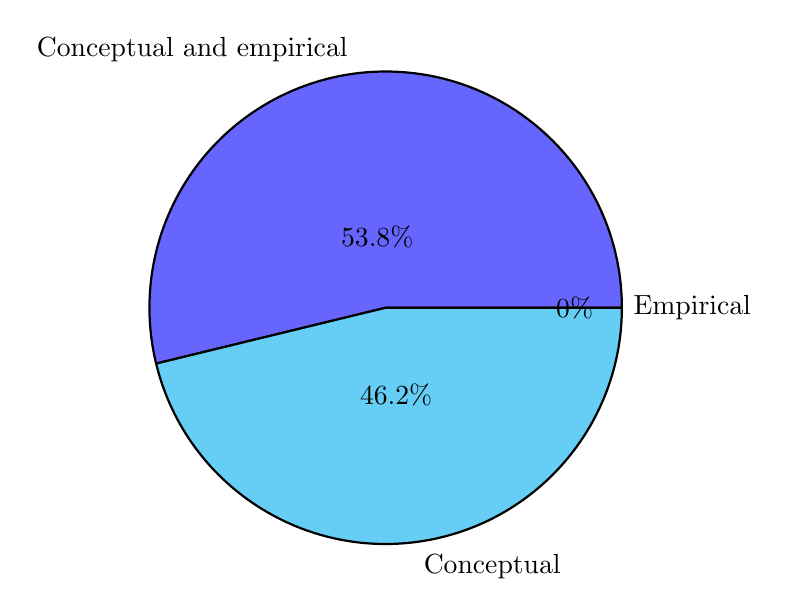
\begin{tikzpicture}
    \pie{53.8/Conceptual and empirical,
        46.2/Conceptual,
        0/Empirical}
    \end{tikzpicture}
    \caption{Conceptual vs empirical}
    \label{fig:concept}
\end{figure}

In the context of a SLR, the distinction between conceptual and empirical papers is important because it provides insights into the type of research that has been conducted in the topic of blockchain and BPM. A conceptual paper introduces a new approach or solution that is based on theoretical or conceptual ideas, and normally does not involve any data collection or experimentation \cite{frizzo-barker_blockchain_2020}. An empirical paper, on the other hand, presents research that is based on data collected through observation or experimentation. From our selected studies none of the papers were purely empirical. As can be seen in Fig. \ref{fig:concept}, half of papers were purely conceptual while the other half were both conceptual and empirical at the same time. In the papers featuring both conceptual and empirical elements, first a new solution is introduced. Then, different experiments are run to measure costs (mostly in terms of Ethereum fees \cite{eth}) or performance in comparison to existing solutions.
\begin{figure}
    \centering
    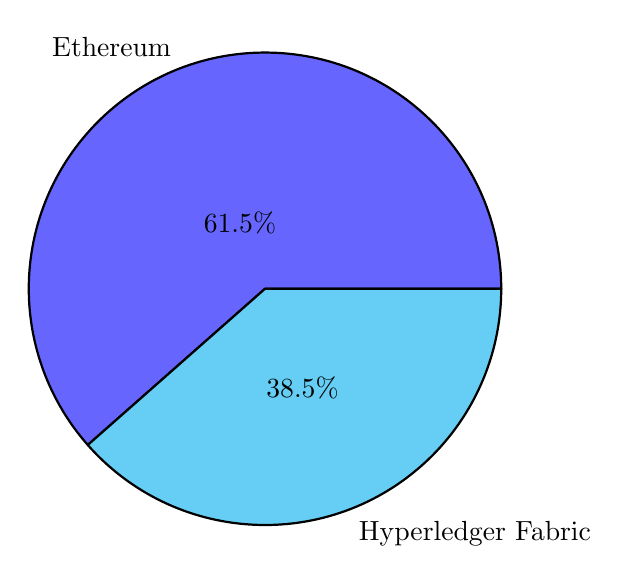
\begin{tikzpicture}
    \pie{61.5/Ethereum,
        38.5/Hyperledger Fabric}
    \end{tikzpicture}
    \caption{Blockchain technology distribution}
    \label{fig:blockchain}
\end{figure}

In our case it is also interesting to see which technologies each study makes use of, which is illustrated on Fig. \ref{fig:blockchain}. As expected Ethereum is the most used platform with 61.5\% of the studies using it. Ethereum is the first and most popular blockchain network that support smart contracts \cite{eth}. The Ethereum network is also permissionless and smart contracts are simple to implement with the Solidity language. In second place comes Hyperledger Fabric \cite{hyperledge}, with 38.5\% of papers developing chaincode solutions. Different from Ethereum, Hyperledger Fabric is a permissioned blockchain platform that is designed for use in enterprise settings \cite{hyperledge}. 
%In contrast to most papers, \citeauthor{ladleif_time_2020} \cite{ladleif_time_2020} was the only study that offered a platform agnostic approach, which they claimed could be applied to Ethereum, Tezos, Hyperledger Fabric and Corda R3.

\subsection{Qualitative analysis and classification results}
In this section, the selected studies are examined in detail and we have grouped them into five different categories, shown in Table \ref{tab:classification}. The categories are based on capabilities that blockchain technologies enables for BPM and challenges faced when implementing such solution. Although the papers are only assigned to one of the categories there is significant overlap between the capabilities supported by the suggested approaches. Here we will only focus on the main topic for each paper.


\setlength{\tabcolsep}{3em}
\begin{table}
    \centering
    \caption{Classification of the selected papers.}
    \begin{tabular}{l c r}
        \hline
        Category & Papers & Number \\
        \hline\hline
        \hyperref[sssec:trust]{Trust Aware} & \cite{alves_exploring_2022, corradini_engineering_2022, fang_workflow_2020, nagano_blockchain_2020, akhtar_blockchain_2020} & 5 (38.4\%)\\
        \hyperref[sssec:flex]{Flexibility} & \cite{corradini_flexible_2022, lopez-pintado_controlled_2022, klinger-upgrade, loukil_decentralized_2021} & 4 (30.8\%)\\
        \hyperref[sssec:temp]{Temporal Constraints} & \cite{abid_modelling_2020, tonga_naha_pupa_2022} & 2 (15.4\%)\\
        \hyperref[sssec:design]{Process Design} & \cite{milani_business_2020, schinle_integration_2020} & 2 (15.4\%)\\
        \hline
    \end{tabular}
    \label{tab:classification}
\end{table}

\subsubsection{Trust Aware}\label{sssec:trust}
Most applications of BC in BPM are introduced into a collaborative setting with multiple parties. Therefore, in these situations the business processes need to be trust aware, meaning to take into account the level of trust between the participants \cite{rosemann2019trust}. \citeauthor{fang_workflow_2020} \cite{fang_workflow_2020} present the Workflow Enactment Service (WES) which allows multiple BPs to interoperate with each other through smart contracts. This eliminates the need for a trusted centralized party. The solution also provides an immutable audit trail for the interoperation of WESs. \citeauthor{alves_exploring_2022} \cite{alves_exploring_2022} suggest a design that combines a Business Process Management System (BPMS) with a blockchain platform into a distributed BPMS to ensure transparent and tamper-proof information sharing among participants. But this solution is later criticized by \citeauthor{nagano_blockchain_2020} \cite{nagano_blockchain_2020} for introducing a Single Point of Trust (SPoT) which a malicious user can attack to falsify related data. They then reveal a system architecture of cross organizational workflow management which eliminates SPoT throughout the workflow lifecycle including defining, executing, and auditing process. \citeauthor{corradini_engineering_2022} \cite{corradini_engineering_2022} intend to target the issue of trust by proposing a novel model-driven methodology for choreography based systems. Their solution, CorChain, relies on a BC infrastructure to enable the trustable execution of a choreography by producing immutable and auditable artefacts. Different from the previous papers, \citeauthor{akhtar_blockchain_2020} \cite{akhtar_blockchain_2020} deals with trust issues stemming from the resources subject to access control policies of multiple organizations. Their approach generates an optimal composite access control policy which enforces all access control policies and minimized policy evaluation cost.

\subsubsection{Flexibility}\label{sssec:flex}
Flexibility refers to the ability of a business to adapt and make changes to its processes quickly and effectively in response to changing requirements \cite{cognini2018business}. Without some degree of flexibility business would not be able to respond to new challenges and opportunities in an ever-changing business environment. Balancing characteristics of blockchain technologies such as immutability with the need for process flexibility has proven to be difficult. \citeauthor{lopez-pintado_controlled_2022} \cite{lopez-pintado_controlled_2022} presents an approach, prototyped in Caterpillar, for dynamic binding of actors to roles in collaborative processes and it also allows actors to control and model subprocesses during runtime. This is accomplished by an off-chain consensus, where all the participants of the collaboration must take part in. Another approach to increasing flexibility was taken by \citeauthor{corradini_flexible_2022} \cite{corradini_flexible_2022}. They propose decoupling the process state, stored in the blockchain as a smart contract, from its execution logic, an off-chain rule-based program. This allows applying runtime changes to a choreography instance without losing the knowledge of the previously exchanged information. Similarly, \citeauthor{klinger-upgrade} \cite{klinger-upgrade} also allow the logic to be updated by decoupling the logic and the data. But differently from the previous solutions they operate only on-chain and rely BPMN collaboration diagram. \citeauthor{loukil_decentralized_2021} \cite{loukil_decentralized_2021} tackles flexibility by proposing an on-chain BPMN interpreter which instantiates and executes processes. This way, they avoid the need for redeployment of the process instance in case of an update to the process model. 

\subsubsection{Temporal Constraints}\label{sssec:temp}
Temporal constraints are the time-based restrictions or rules that govern the execution of a business process. These constraints define the start and end times of activities, the duration of activities, and the time dependencies between activities. Most blockchain technologies have difficulties in ensuring the accurate application of time-based restrictions across a decentralized system since the they do not allow access to an external or internal clock  \cite{ladleif_time_2020}. \citeauthor{abid_modelling_2020} \cite{abid_modelling_2020} tackle the uncertainty of the time it takes to reach transaction finality, which can vary from minutes to hours. They propose an extension to the Caterpillar tool to enable the transformation of temporal constraints for BPMN to smart contract code. In the same vein, \citeauthor{tonga_naha_pupa_2022} \cite{tonga_naha_pupa_2022} seeks to solve the shortcomings of Caterpillar by introducing an extension called Pupa. Pupa not only translates time events but also inclusive gateways to smart contracts.  


\subsubsection{Process Design}\label{sssec:design}
This category includes papers which concern themselves broadly with the design (and modeling) activity of BPM. Designing and modeling processes for blockchain technologies comes with its own challenges because of the idiosyncrasies of the technology. Although all studies selected touch on this topic, the following two papers provide new perspectives which are worth highlighting. \citeauthor{milani_business_2020} \cite{milani_business_2020} analyze the business process redesign (BPR) principles in light of their applicability to blockchain-based solutions. They adapt the best practices of BPR for BC and also explore their applicability with a case study. On a different direction than most papers, \citeauthor{schinle_integration_2020} \cite{schinle_integration_2020} introduces a reverse translator which takes arbitrary chaincode and translates it to a BPMN 2.0 model. Their aim is to enable monitoring of processes defined within a chaincode while reducing the required knowledge about Hyperledger Fabric.
\section{Discussion}
In this section we discuss the answers to our research questions that we derived from the selected literature. Furthermore, we present some possible directions for future research.

\subsection{RQ1: How can BPM take advantage of blockchain technologies?}
As was the case with the previous surveys \cite{mendling_blockchains_2018, garcia-garcia_using_2020, lauster}, blockchain technologies are still seen through the lens of collaboration and inter-organizational processes. Most of the solutions presented cite removing intermediaries and increasing trust between participants as the main motivator. Therefore, they leverage the ability of blockchain technologies to facilitate secure, decentralized, and transparent collaboration between multiple parties. Additionally, smart contract capabilities within blockchain can automate and enforce the execution of business processes, reducing manual intervention and improving efficiency. 

\subsection{RQ2: What are the top challenges and risks associated with integrating blockchain in BPM?}
Some of the challenges related to the inherent shortcomings of the technology have been addressed by the selected papers. In this review, two main challenges are handled: (1) the lack of ability to gather time information or perform timed events which hinders the enforcement of temporal constraints, and (2) the immutability of deployed smart contracts making process flexibility more complex to implement. Aside from these issues, the cost, performance, and scalability of the present solutions are mentioned but mostly as a secondary concern. 

\subsection{RQ3: Which applications of blockchain in BPM have been proposed and how are they evaluated?}
As this review and previous reviews have demonstrated, several applications for BPM have been proposed and implemented. Some shown in the selected papers are: Pupa, ChorChain, FlexChain, CoBuP and other unnamed solutions. Some of these solutions are extensions to Caterpillar, while others are standalone solutions. The solutions are mostly evaluated through use cases. In some studies, they are also evaluated using cost or performance analysis by running experiments. 

\subsection{Future Research Direction}
Although much effort has been put into the field linking BC and BPM, it is still in its early stages and there is much room for further research and development. The following research directions can be used as a guide for any future studies. 
\begin{description}
  \item[Performant Blockchains] When choosing a permissonless blockchain network all studies decided for Ethereum. While the Ethereum platform has many advantages, currently it is not cost efficient nor does it have high performance in comparison to other blockchain platforms. The use of cheaper and faster blockchains, such as Solana, will most probably be of high interest in the future \cite{pierro2022can}.   
  \item[Security] Blockchain solutions are endorsed as highly secure because of their cryptographic properties. This security is completely predicated on the secrecy of the user's private key. These keys are usually stored as a random set of characters, a secret phrase or a qr-code making it trivial for users to lose them. In a worst case scenario, these key can be uncovered by a malicious third party. Studies discussing the security implications of users managing their own private keys in relation to BC in BPM are needed. Another important security concern that needs further research is the handling of logical errors in smart contracts. In a permissionless network, these errors can be easily exploited and incur great financial damage \cite{atzei2017survey}.    
  \item[Human factors] Most studies only focus on the technical side of the problem. For the field to achieve its full potential it is crucial to understand how human factors impact the success of blockchain-based BPM. Although a large number of people have heard or own cryptocurrencies, they are still hesitant when presented with blockchain-based solutions \cite{alshamsi2022systematic}. Future research can explore ways to overcome this hesitancy, as well as ways to engage and motivate users to adopt this new technology.

  \item[Empirical Studies] As Table \ref{fig:concept} suggests, there is a lack of empirical studies in the field. The selected studies were either conceptual or conceptual with some empirical evaluation of the presented approach. In general, more empirical research is needed in the field to provide evidence for future decision-making.
\end{description}
\section{Conclusion}
With this paper, we have performed a SLR linking blockchain and BPM. We identified a total of 13 relevant primary studies. These studies were selected from 1659 recent publications related to the topic. We ran a quantitative analysis by first showing the geographic distribution of the various authors. Then we classified the studies in conceptual, empirical or both. We also illustrated which blockchain technology the studies considered. Most of the implementations being accomplished with Solidity for the Ethereum platform. For our qualitative analysis, we classified the papers into 4 main groups according to capability/challenge: trust aware, flexibility, temporal constraints and process design. It was found that blockchain offers a great solution to address trust concerns by eliminating the need for a central party and creating auditable, tamper-proof artefacts (such as data or logs). New solutions were introduced to challenges mentioned in previous reviews, such as lack of flexibility and inability to enforce temporal constraints. In the future, we propose (1) considering more performant blockchain platforms, (2) addressing security more in-detail, (3) studying human factors such as adoption, and (4) performing more empirical research to enable decision-making.     

% \section{First Section}
% \subsection{A Subsection Sample}
% Please note that the first paragraph of a section or subsection is
% not indented. The first paragraph that follows a table, figure,
% equation etc. does not need an indent, either.

% Subsequent paragraphs, however, are indented.

% \subsubsection{Sample Heading (Third Level)} Only two levels of
% headings should be numbered. Lower level headings remain unnumbered;
% they are formatted as run-in headings.

% \paragraph{Sample Heading (Fourth Level)}
% The contribution should contain no more than four levels of
% headings. Table~\ref{tab1} gives a summary of all heading levels.

% \begin{table}
% \caption{Table captions should be placed above the
% tables.}\label{tab1}
% \begin{tabular}{|l|l|l|}
% \hline
% Heading level &  Example & Font size and style\\
% \hline
% Title (centered) &  {\Large\bfseries Lecture Notes} & 14 point, bold\\
% 1st-level heading &  {\large\bfseries 1 Introduction} & 12 point, bold\\
% 2nd-level heading & {\bfseries 2.1 Printing Area} & 10 point, bold\\
% 3rd-level heading & {\bfseries Run-in Heading in Bold.} Text follows & 10 point, bold\\
% 4th-level heading & {\itshape Lowest Level Heading.} Text follows & 10 point, italic\\
% \hline
% \end{tabular}
% \end{table}


% \noindent Displayed equations are centered and set on a separate
% line.
% \begin{equation}
% x + y = z
% \end{equation}
% Please try to avoid rasterized images for line-art diagrams and
% schemas. Whenever possible, use vector graphics instead (see
% Fig.~\ref{fig1}).

% \begin{figure}
% 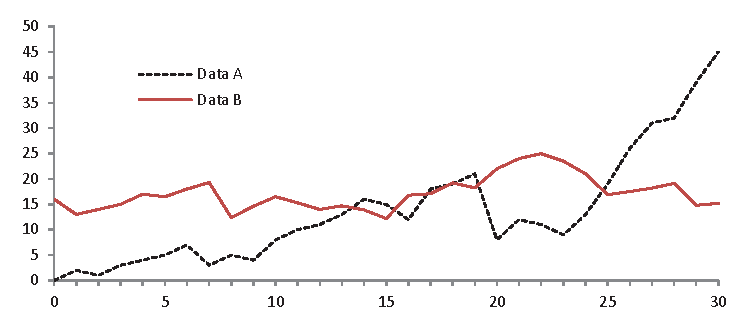
\includegraphics[width=\textwidth]{fig1.eps}
% \caption{A figure caption is always placed below the illustration.
% Please note that short captions are centered, while long ones are
% justified by the macro package automatically.} \label{fig1}
% \end{figure}

% \begin{theorem}
% This is a sample theorem. The run-in heading is set in bold, while
% the following text appears in italics. Definitions, lemmas,
% propositions, and corollaries are styled the same way.
% \end{theorem}
% %
% % the environments 'definition', 'lemma', 'proposition', 'corollary',
% % 'remark', and 'example' are defined in the LLNCS documentclass as well.
% %
% \begin{proof}
% Proofs, examples, and remarks have the initial word in italics,
% while the following text appears in normal font.
% \end{proof}
% For citations of references, we prefer the use of square brackets
% and consecutive numbers. Citations using labels or the author/year
% convention are also acceptable. The following bibliography provides
% a sample reference list with entries for journal
% articles~\parencite{garcia-garcia_using_2020}, an LNCS chapter~\cite{ref_lncs1}, a
% book~\cite{ref_book1}, proceedings without editors~\cite{muller_silver_2020},
% and a homepage~\cite{ref_url1}. Multiple citations are grouped
% \cite{ref_article1,ref_lncs1,ref_book1},
% \cite{ref_article1,ref_book1,ref_proc1,ref_url1}.
%
% ---- Bibliography ----
%
% BibTeX users should specify bibliography style 'splncs04'.
% References will then be sorted and formatted in the correct style.
%
%\bibliographystyle{splncs04}

\printbibliography{}
% \begin{thebibliography}{8}
% \bibitem{ref_article1}
% Author, F.: Article title. Journal \textbf{2}(5), 99--110 (2016)

% \bibitem{ref_lncs1}
% Author, F., Author, S.: Title of a proceedings paper. In: Editor,
% F., Editor, S. (eds.) CONFERENCE 2016, LNCS, vol. 9999, pp. 1--13.
% Springer, Heidelberg (2016). \doi{10.10007/1234567890}

% \bibitem{ref_book1}
% Author, F., Author, S., Author, T.: Book title. 2nd edn. Publisher,
% Location (1999)

% \bibitem{ref_proc1}
% Author, A.-B.: Contribution title. In: 9th International Proceedings
% on Proceedings, pp. 1--2. Publisher, Location (2010)

% \bibitem{ref_url1}
% LNCS Homepage, \url{http://www.springer.com/lncs}. Last accessed 4
% Oct 2017
% \end{thebibliography}
\end{document}
